\documentclass{report}

\usepackage{enumitem}
\usepackage{hyperref}
\usepackage{listings}
\usepackage{color}
\usepackage{xcolor}
\usepackage{tikz}
\usepackage[utf8]{inputenc} 
\usepackage[T1]{fontenc}
\usepackage{graphicx}
\usepackage{multirow}
\usepackage{booktabs}
\usepackage{array}
\usepackage{changepage}



\lstdefinestyle{customasm}{
    belowcaptionskip=1\baselineskip,
    frame=single, 
    frameround=tttt,
    xleftmargin=\parindent,
    language=[x86masm]Assembler,
    basicstyle=\footnotesize\ttfamily,
    commentstyle=\itshape\color{green!60!black},
    keywordstyle=\color{blue!80!black},
    identifierstyle=\color{red!80!black},
    tabsize=4,
    numbers=left,
    numbersep=8pt,
    stepnumber=1,
    numberstyle=\tiny\color{gray}, 
    columns = fullflexible,
}

\newcommand{\thickhline}{\noalign{\hrule height 1.2pt}}

\title{Static Binary Rewriting for AFL-style Edge Coverage Instrumentation}
\author{Scandroglio Edoardo}
\date{\today}
\begin{document}
    \maketitle
    \tableofcontents
    \chapter{Introduction}
        Fuzzing is nowadays one of the most popular software testing and automated vulnerability discovery techniques.
        Among all fuzzing techniques, one of the most widely used is grey-box fuzzing, which relies on coverage-guided input mutation.
        The idea is to discover which portions of the target application are visited during execution,
            in order to generate inputs that maximize the number of instructions explored and, consequently, the number of vulnerabilities discovered during fuzzing.
        In particular, the most commonly used approach is to track Edge Coverage, i.e., to keep track of which branches are taken (or not taken).
        If the source code is not available, adding Edge Coverage instrumentation relies on two main techniques:
        \begin{itemize} 
            \item \textit{Static Binary Instrumentation}: rewrites the target application before execution.
            \item \textit{Dynamic Binary Instrumentation}: rewrites instructions during execution.
        \end{itemize}
        Dynamic Binary Instrumentation introduces significant overhead (roughly 100--400\%) and, due to this, wastes a considerable amount of resources and time.
        On the other hand, Static Binary Instrumentation in the absence of source code is difficult, because it is based
            on modifying a binary without recompiling it. A static binary rewriter must preserve the correctness of the original binary.
        In this thesis I will focus on Static Binary Instrumentation. The current state-of-the-art could be represented by:
        \begin{itemize}
            \item \textbf{ZAFL} is a Static Binary Instrumentation tool that inserts AFL-style edge coverage instrumentation inside a binary while optimizing the code.
            \item \textbf{Retrowrite} : create a "reassembleable assembly" adding labes instead of references and make instrumentation easier, because the is not tje risk of break these references.   
        \end{itemize}
        
    Retrowrite main drawback is that supports only PIE non-stripped binaries and does not provide an edge coverage instrumentation mechanism, relying instead on afl-gcc.
    ZAFL, on the other hand, achieves overhead close to compile-time instrumentation, but remains fragile against obfuscated or anti-analysis binaries.
    This is reported in the paper \textit{Robust, Efficient, and Widely Available Greybox Fuzzing for COTS Binaries with System Call Pattern Feedback}.
    Moreover, ZAFL instruments the shared-map update as a call to a function, rather than placing the update instructions inline within each basic block.

    My approach is to implement an edge coverage instrumentation tool that is compatible with AFL++ and relies on the GRAPE static binary rewriter.
    The instructions must be placed inline within each basic block and must work on both stripped and non-stripped binaries.

    This approach is implemented through two main stages:
    \begin{itemize}
        \item First, I extend the binary by inserting a dynamic dependency to a previously compiled shared object, and by inserting new sections into the binary along with new relocation entries.
        \item Second, I parse the newly obtained binary with GRAPE and then insert the shared-memory update instructions inline at the beginning of each basic block.
    \end{itemize}
    The shared object contains a forkserver that implements the AFL++ communication protocol.

    In only one of the conducted tests did the software fail to instrument the target binary. However, on some targets the instrumentation causes a segmentation fault when accessing the .bss section, due to the reorganization of binary segments performed by the lief library used to insert the dynamic dependency. The performance obtained on the tested targets through AFL++ is comparable to that of source-code instrumentation performed by AFL++, and slightly better than ZAFL.
             
    \begin{itemize}
        \item A static rewriting pipeline that instruments stripped and non-stripped binaries with AFL-style edge coverage without requiring source or symbol information.
        \item A technique for handling indirect control flow that preserves the correctness of binaries.
\end{itemize}
    
        \chapter{Motivation}
            \section{Problem Statement}
                The problem I aim to solve is to statically instrument a binary with edge coverage instructions
                in a way that is compatible with the AFL++ fuzzer, that adds as little overhead as possible with respect to
                the overhead added by compile-time instrumentation, and that preserves the correctness of the binary.\\
                This is important because lower instrumentation overhead means more executions per second during fuzzing,
                 which allows a larger portion of the input space to be explored in the same amount of time,
                 increasing the probability of discovering a given vulnerability.

            \section{State of the Art}
                The state of the art in terms of fuzzers is represented by the AFL++ fuzzer, which includes
                    state-of-the-art techniques for seed selection, queue culling, and performance.
                However, AFL++ relies on instrumentation added at compile time. In the absence of source code,
                    the state of the art is represented by several alternatives:
                \begin{itemize}
                    \item \textbf{AFL in QEMU mode}: A Dynamic Binary Instrumentation approach based on the QEMU virtualized environment.
                            AFL uses QEMU in user-mode emulation. In this mode, QEMU translates guest machine code into
                            intermediate representation blocks called Translation Blocks (TBs). AFL patches this translation mechanism.
                            Every time QEMU translates a new TB, the patching mechanism appends the shared-map update instructions
                            at the end of it, before this code is executed.
                            This technique introduces prohibitive overhead, significantly reducing the number of inputs that
                            can be tested. 
                    \item \textbf{AFL-Dyninst}: A Static Binary Instrumentation approach based on the Dyninst binary rewriter.
                            The Dyninst instrumentation engine works through trampolines, which degrade execution performance and introduce overhead
                            due to the required context switches.
                            Moreover, every trampoline call must preserve the context: registers and flags must be saved before the trampoline
                            is entered and restored after it returns.
                    \item \textbf{RetroWrite}: This tool performs symbolic lifting on the code, replacing every reference
                        discovered during disassembly with a symbolic label. Doing this allows instructions to be added without
                        modifying the references, achieving reassembleable assembly.
                        While RetroWrite can add ASan instrumentation, it cannot natively add AFL-style edge coverage instructions.
                        To do so, the lifted assembly must be instrumented with the afl-gcc tool in order to produce the patched binary.
                        Moreover, community-reported issues document missing instrumentation points when
                        RetroWrite's symbolized output is compiled through afl-gcc, caused by a mismatch between RetroWrite's
                        label-naming convention and afl-as's basic-block detection heuristics.
                        Finally, RetroWrite only works with PIE, non-stripped binaries.
                    \item \textbf{ZAFL}: ZAFL performs a first step of binary analysis and Intermediate Representation (IR) reconstruction.
                            From the IR, it performs live-variable and CFG analyses, based on which it carries out optimization steps
                            capable of optimizing the CFG before actually adding the edge coverage instrumentation.
                            The shared-map update instructions are added as function calls inside the basic blocks,
                            causing performance degradation due to the associated context switches.
                \end{itemize}

            \section{Goals and Challenges}
                The main goal of this thesis is to develop a tool capable of inline, static edge-coverage instrumentation
                that preserves binary correctness while achieving performance comparable to compile-time instrumentation.\\
                This approach involves several challenges, mainly related to preserving the binary's correctness and behavior.
                Preserving all data/code references is considered a particularly hard problem, especially in obfuscated binaries.
                In fact, although GRAPE correctly reconstructs all the references, binary layout preservation
                has been the main challenge, mainly because the binary analysis library tends to modify the binary's segment layout.


        \chapter{Approach}
            \section{Approach Overview}
                The overall approach is based on the AFL shared-map update, which can be summarized with the following two instructions:\\
                \textit{\lstinline|shared_map[current^previous]++;|}\\
                \textit{\lstinline|current>>1;|}\\  
                where \texttt{current} and \texttt{previous} are the IDs of the basic blocks between which the transition occurs.
                A forkserver is injected into the target binary by adding a dynamic dependency to a shared library containing the forkserver's code.
                The forkserver implements the communication protocol with the fuzzer.
                \\
                The overall instrumentation approach can be divided into the following steps:
                \begin{enumerate}
                    \item Modify the ELF by adding a dynamic dependency, new sections, and new relocations.
                    \item Analyze the new ELF, reconstruct the CFG, and discover the main address.
                    \item Insert the initial instrumentation at \texttt{main}, needed to initialize previous basic block ID.
                    \item Search for instrumentation points.
                    \item Instrument the previously found instrumentation points.
                    \item Adjust the internal references of the ELF.
                    \item Write the patched file.
                \end{enumerate}
                \begin{figure}[ht]
                    \centering
                    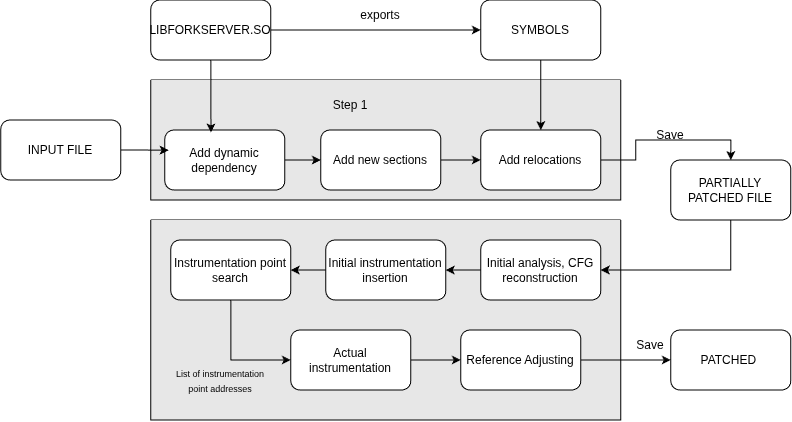
\includegraphics[width=\textwidth]{images/OverallFunctioning.png}
                    \caption{Overall Functioning}
                \end{figure}
            \section{Approach Details}
                \begin{itemize}
                    \item \textbf{Step 1 -- Dynamic dependency, sections, and relocations insertion}: Add a dynamic dependency to the shared object \textit{libforkserver.so}.
                                This shared object contains the forkserver and implements the communication protocol with AFL/AFL++.
                                Moreover, during this step, two new sections are added to the binary:
                                \begin{itemize}
                                    \item \textit{.mygot}: contains the relocated symbols from the shared object. This is a pointer to the shared map initialized in the libforkserver.so object and a pointer to forkserver function;
                                    \item \textit{.mydata}: a section used as temporary variable storage. It contains space to save the \texttt{rax} register, the value of the previous basic block ID, and the dereferenced address of the shared map.
                                \end{itemize}
                    \item \textbf{Step 2 -- Initial analysis}: The CFG is reconstructed, and by analyzing it the main address
                                    can be found in both the stripped and non-stripped cases.
                                    The addresses of the functions that should not be instrumented (such as \texttt{frame\_dummy} and other setup functions) are found and excluded from later instrumentation.
                    \item \textbf{Step 3 -- Initial instrumentation}: Through the relocated symbols, the address of the forkserver function is found and the forkserver is invoked. 
                                    The previous basic block ID is initialized to a random value and stored into the \textit{.mydata} section 
                                    and then the address of the shared map is obtained from the relocated symbol and stored, for efficiency reasons, into \textit{.mydata}.
                                    The assembly instrumented in this initial part can be summarized as follows:
                                    \begin{lstlisting}[style=customasm, caption={Initial Instrumentation Code}, label=Initial Instrumentation Code]
push rsi
push rdi
mov rax, QWORD PTR[rip + offset_to_relocated_forkserver_function]
mov rax, [rax]
call rax
mov WORD PTR[rip + offset_to_previous_saved_ID], random_int
lea rax, [rip + offset_to_relocated__afl_area_ptr]
mov rax, QWORD PTR [rax]
mov rax, QWORD PTR [rax]
mov QWORD PTR[rip + offset_to_saved_shared_memory_address], rax
                                    \end{lstlisting}
                
                \item \textbf{Step 4 -- Instrumentation point search}: Starting from the main address, a Depth-First Search is executed
                                    to obtain all the basic blocks reachable from it.
                                    Every time a new basic block is found, before it is inserted into the list of basic blocks that need to be instrumented,
                                    it is checked against the previously determined list of functions to be excluded from instrumentation.
                                    It is also checked whether the last instruction of the previous basic block is a call.
                                    Since a call is always taken, the following basic blocks are not instrumented.
                \item \textbf{Step 5 -- Actual instrumentation}: For each basic block previously found, its first address is instrumented.
                    Before actually inserting the instructions, the offset to \textit{.mydata} has to be computed relative to the instrumentation address.
                    The inserted instructions can be summarized as follows:
                    \begin{lstlisting}[style=customasm, caption={Shared Map Update Code}, label=Shared Map Update Code]
mov QWORD PTR[rip + offset_to_saved_rax], rax
movzx rax, WORD PTR[rip + offset_to_previous_saved_ID]        
xor ax, random_current_basic_block_ID
add rax, QWORD PTR[rip + offset_to_saved_shared_memory_address]
inc BYTE PTR[rax]
mov WORD PTR[rip + offset_to_precedent_bb_saved], right_shifted_current_ID
mov rax, QWORD PTR[rip + offset_to_saved_rax]
                    \end{lstlisting}       
                    This snippet of assembly performs the aforementioned shared-map update:\\
                     \textit{\lstinline|shared_map[current^previous]++;|}\\
                    \textit{\lstinline|current>>1;|}       
        
                \item \textbf{Step 6 -- Reference adjustment}: All the instructions of each basic block are scanned in search of
                    displaced references, which, when found, are adjusted to their new, correct value. 
                    Then is checked (and eventually corrected) any mismatch between the ELF layout and the ELF header
                \item \textbf{Step 7 -- Write the new patched ELF}
            \end{itemize}

        \chapter{Implementation Details}
            \section{System Architecture}
                There are two main files:
                \begin{itemize}
                    \item \textbf{instrumentator.py}: contains all the logic used to instrument the target application.\\
                    \item \textbf{libforkserver.so}: This library contains the communication protocol used with the fuzzer, along with the forkserver.
                        It can work both in standalone mode (without an actual fuzzer) and in normal mode.
                        In standalone mode, the map is initialized as a local memory region instead of a shared memory region.
                        The library also exports the symbols to be relocated inside the target application.\\
                \end{itemize}       

            \section{System Details}
                \begin{itemize}
                    \item \textbf{instrumentator.py}: For \textit{Step 1}, the lief Python library is used to add the dynamic dependency, the new sections, and the relocations.
                            For all the other steps, the GRAPE framework is used, which provides API calls to add, remove, and replace an instruction at a specific address in the .text section of the ELF.
                    \item \textbf{libforkserver.so}: The library contains a constructor executed before the target's \texttt{main}.
                        During the execution of the constructor, it accesses two environment variables to configure the mode in which the forkserver must run. Specifically:
                        \begin{itemize}
                            \item \textit{\_\_AFL\_SHM\_ID}: set by the fuzzer, contains the ID of the shared memory.
                            \item \textit{\_\_AFL\_PLUSPLUS}: equal to one if the AFL++ communication protocol is to be used; otherwise, the AFL communication protocol is used.
                        \end{itemize}
                        The forkserver is executed by the main of the target. Three different function pointers could be used to run the forkserver in different mode:
                        \begin{itemize}
                            \item \textit{standalone mode}: The shared map is allocated locally and there is no communication with the fuzzer.
                            \item \textit{AFL mode}: The shared map is obtained through the shared memory ID from the environment variable.
                            \item \textit{AFL++ mode}: Same as the previous, but the communication protocol is different.
                        \end{itemize}
                        Communication with the fuzzer happens unidirectionally through two different file descriptors created by the fuzzer:
                        \begin{itemize}
                            \item \textit{forkserver\_read (fd 198)}: used by the forkserver to read a message from the fuzzer.
                            \item \textit{forkserver\_write (fd 199)}: used by the forkserver to write a message to the fuzzer.
                        \end{itemize}

                        Inside libforkserver.so the \textit{\_\_afl\_area\_ptr} and \textit{\_\_forkserver\_start\_ptr} symbols are declared with \\\textit{\_\_attribute\_\_((visibility("default")))}, and therefore visible outside the library.
                        This symbols are then relocated inside the target, where they are read/updated by it.
                        \begin{itemize}
                            \item \textit{\_\_afl\_area\_ptr}: contains the address of the shared map that needs to be updated by the target. 
                            \item \textit{\_\_forkserver\_start\_ptr}: contains the pointer to the forkserver function selected during constructor execution of the shared object.
                        \end{itemize}
                        

                        The communication protocol differs slightly between the AFL and AFL++ modes. During fuzzer execution, the interaction between fuzzer, target, and forkserver can be represented as follows.
                        \begin{figure}[ht]
                            \centering
                            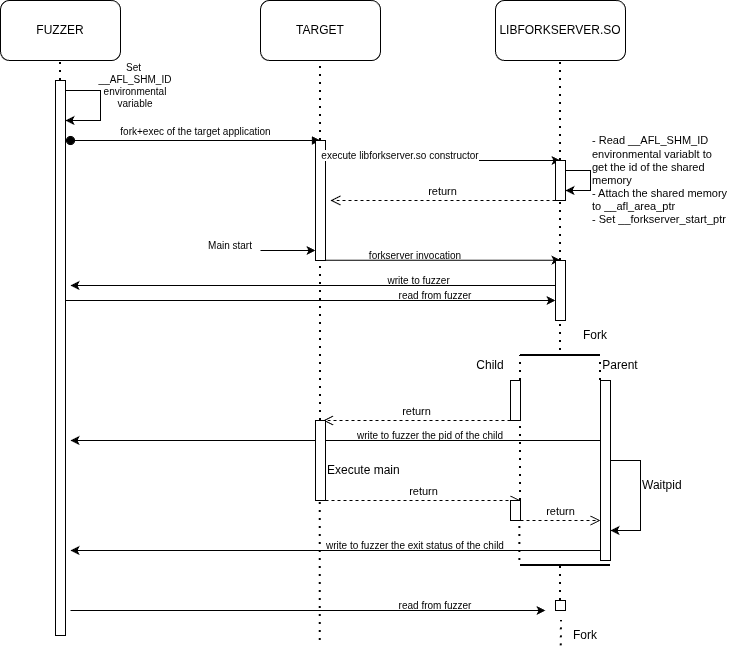
\includegraphics[width=\textwidth]{images/AFLForkServerProtocol.png}
                            \caption{AFL fuzzer execution}
                        \end{figure}
                        \begin{figure}[ht]
                            \centering
                            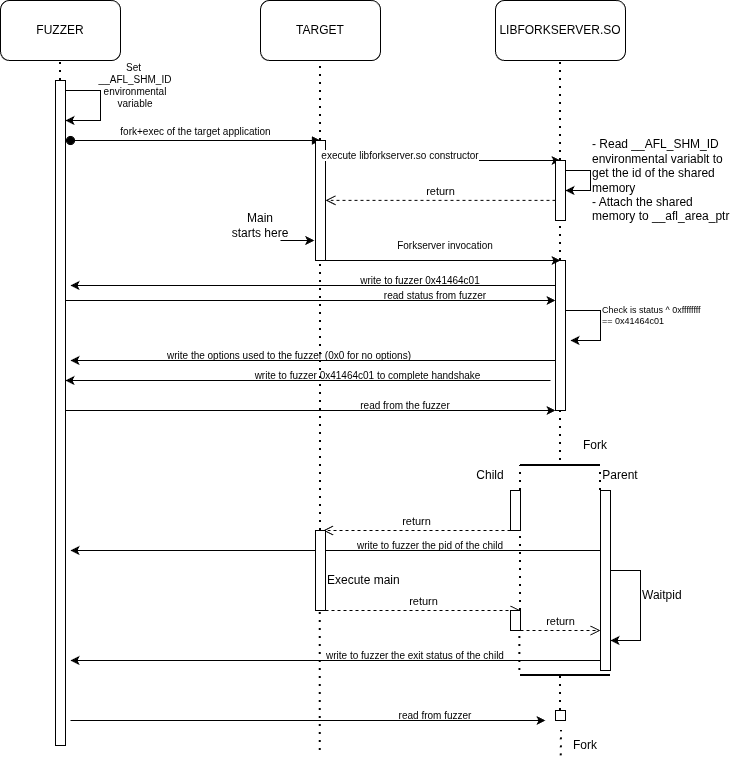
\includegraphics[width=\textwidth]{images/AFLPlusPlusForkServerProtocol.png}
                            \caption{AFL++ fuzzer execution}
                        \end{figure}

                \end{itemize}


        \chapter{Experimental Validation}
            \section{Goals}
                \begin{itemize}
                    \item \textbf{Goal I} : Show that the rewriter produce correct binaries
                    \item \textbf{Goal II} : Show taht instrumentation overhead is competitive with other binary only rewriters and lower
                        than dynamic binary translator.
                \end{itemize}
            \section{Dataset}
                The dataset used for testing is composed of the original LAVA-M testbench binaries (\textit{base64, md5sum, uniq, who}) 
                already injected with synthetic vulnerabilities.
                All the binaries are compiled with GCC 5.4.0, all 4 unstripped.
                The \textit{md5sum} has been downloaded already corrupted. Both afl in qemu mode and the tool developed fails to instrument it.
                Onlu ZAFL success in instrument it mainly because ZAFL perform an optimization step that probably fix the error.

            \section{Experimental Setup}
                All the experiments are done with AFL++ version 5.03c and made across 24 hours fuzzing campaign with 3 different repetitions per binary tested.
            \section{Experiment I - Correctness}
                For \textit{base64} and \textit{uniq} binaries the behavior is preserver after the instrumentation.
                Running these 2 binaries in standalone mode produce the same output as using the non instrumented version.\\
                \textit{who} binary instead fail to preserve behavior. Infact the instrumentation cause a Segmentation Fault at each run. 

            \section{Experiment II - Instrumentation Overhead}
                \begin{table}[h]
                    \centering
                    \begin{adjustwidth}{-4.7cm}{-4.7cm}
                        \resizebox{\paperwidth}{!}{
                            \begin{tabular}{|c|c!{\vrule width 1.2pt}c|c|c!{\vrule width 1.2pt}c|c|c!{\vrule width 1.2pt}c|c|c|}
                            \hline
                             & & \multicolumn{3}{c!{\vrule width 1.2pt}}{afl} & \multicolumn{3}{c!{\vrule width 1.2pt}}{mine} & \multicolumn{3}{c|}{zafl} \\
                            \hline
                            & & run1 & run2 & run3 & run1 & run2 & run3 & run1 & run2 & run3 \\
                            \thickhline
                            \multirow{4}{*}{base64} 
                            & execs\_per\_sec   & 398.49   & 444.98   & 351.77 
                                                & 1703.45  & 1738.99  & 1842.27
                                                & 2281.00  & 1772.18  & 1687.38\\
                            \cline{2-11}
                            & execs\_done   & 34429329   & 38446221   & 30392855 
                                            & 147177902  & 150249117  & 159172058
                                            & 197078290  & 153115984  & 145790015\\
                            \cline{2-11}
                            & edges\_found  & 690 & 690 & 690 
                                            & 358 & 370 & 358
                                            & 640 & 640 & 640\\
                            \cline{2-11}
                            & saved\_crashes    & 7  & 3  & 2 
                                                & 12 & 41 & 11
                                                & 11 & 8  & 13\\
                            \thickhline
                            \multirow{4}{*}{md5sum} 
                            & execs\_per\_sec   & \textcolor{red}{x} & \textcolor{red}{x} & \textcolor{red}{x} 
                                                & \textcolor{red}{x} & \textcolor{red}{x} & \textcolor{red}{x} 
                                                & 515.09& & \\
                            \cline{2-11}
                            & execs\_done   & \textcolor{red}{x} & \textcolor{red}{x} & \textcolor{red}{x} 
                                            & \textcolor{red}{x} & \textcolor{red}{x} & \textcolor{red}{x}
                                            & 44503697& & \\
                            \cline{2-11}
                            & edges\_found  & \textcolor{red}{x} & \textcolor{red}{x} & \textcolor{red}{x} 
                                            & \textcolor{red}{x} & \textcolor{red}{x} & \textcolor{red}{x}
                                            & 9& & \\
                            \cline{2-11}
                            & saved\_crashes    & \textcolor{red}{x} & \textcolor{red}{x} & \textcolor{red}{x} 
                                                & \textcolor{red}{x} & \textcolor{red}{x} & \textcolor{red}{x}
                                                & 846& & \\
                            \thickhline
                            \multirow{4}{*}{uniq} 
                            & execs\_per\_sec   & 567.81  & 576.57   & 577.17 
                                                & 1758.61 & 1399.39  & 1864.43 
                                                & 2023.72 & 1614.07  & 1885.92\\
                            \cline{2-11}
                            & execs\_done   & 49058377  & 49815928   & 49867759 
                                            & 151943556 & 120907581  & 161086939 
                                            & 174849429 & 139455948  & 162943673\\
                            \cline{2-11}
                            & edges\_found      & 473 & 473 & 473 
                                                & 242 & 242 & 242
                                                & 443 & 443 & 443\\
                            \cline{2-11}
                            & saved\_crashes    & 2 & 0 & 0 
                                                & 0 & 0 & 0
                                                & 0 & 0 & 0\\
                            \thickhline
                            \multirow{4}{*}{who} 
                            & execs\_per\_sec   & 225.11 & & 
                                                & \textcolor{red}{x} & \textcolor{red}{x} & \textcolor{red}{x} 
                                                & 456.42 & & \\
                            \cline{2-11}
                            & execs\_done   & 19449595 & & 
                                            & \textcolor{red}{x} & \textcolor{red}{x} & \textcolor{red}{x} 
                                            & 39434809 & & \\
                            \cline{2-11}
                            & edges\_found      & 13770 & & 
                                                & \textcolor{red}{x} & \textcolor{red}{x} & \textcolor{red}{x} 
                                                & 14044 & & \\
                            \cline{2-11}
                            & saved\_crashes    & 0 & & 
                                                & \textcolor{red}{x} & \textcolor{red}{x} & \textcolor{red}{x} 
                                                & 2 & & \\
                            \hline
                            \end{tabular}
                        }
                    \end{adjustwidth}
                    \caption{Fuzzing statistics over 24 hours fuzzing campaing on LAVA-M dataset}
                    \label{table:5.1}
                \end{table}
                \textit{The empty cells are there because, since there is not a comparison with the tool discussed in this thesis, the experiment had not been done}
                \begin{table}[h]
                    \centering
                    \begin{tabular}{|c!{\vrule width 1.2pt}c|c!{\vrule width 1.2pt}c|c!{\vrule width 1.2pt}c|c!{\vrule width 1.2pt}}
                        \hline
                            & \multicolumn{2}{c!{\vrule width 1.2pt}}{base64} & \multicolumn{2}{c!{\vrule width 1.2pt}}{uniq} & \multicolumn{2}{c!{\vrule width 1.2pt}}{who}\\
                            \hline
                            & mine & zafl & mine & zafl & mine & zafl \\
                            \hline
                            file\_size[MByte]   & 8,25228  & 0,137459 
                                                & 8,256376 & 0,149747 
                                                & 8,62092  & 1,718515\\
                            \hline
                            avg\_execs\_per\_sec    & 1761.57 & 1913.52 
                                                    & 1674.14 & 1841.24
                                                    & \textcolor{red}{x}& 456.42\\
                            \hline
                    \end{tabular}
                    \caption{Instrumented binaries statistics}
                \end{table}

        \chapter{Limitations}
            The main limitation is that the developed software fails to preserve the correctness of the target binary when the lief library changes the ELF layout, for example by altering the segment layout.
            For instance, when the dynamic dependency is added to the binary, some of the sections are modified. Specifically:
            \begin{itemize}
                \item \textit{.dynstr}: the string 'libforkserver.so' has to be placed inside the dynamic string section.
                \item \textit{.dynamic}: lief adds a DT\_NEEDED entry that points to the newly added string in \textit{.dynstr}.
            \end{itemize}
            If, during either of these two additions, lief exceeds the available space of the segment containing the grown section, it reorganizes the segments.
            This causes a complete displacement of the data sections (such as \textit{.bss, .data, .rodata}, etc.) without a corresponding fix to the instructions that reference these data sections.\\
            Another limitation is that this pipeline relies heavily on the Linux ELF binary format and fails to instrument Windows PE binaries.
        \chapter{Future Works}
            Improve binary correctness after instrumentation in such a way that the original behavior is preserved.
            Moreover some of the state-of-the-art techniques that mitigate hash collision could be implemented into the framework in order to improve fuzzing effectiveness.

        \chapter{Conclusion}

            The goal of this thesis was to develop a static binary instrumentator that uses GRAPE as binary rewrite framework
            capable of inserting AFL-style edge coverage instructions inline within each basic block without relying of source of or symbol table, while
            remains compatible with AFL++ fuzzer. This instrumentation has to add as less overheads as possible with respect to compile time instrumentation.\\

            The developed approach rely on \textit{lief} python library to add needed sections, libraries and relocation and GRAPE
            to actually insert edge-coverage instrumentation while reconstruct references, both in PIE and nonPIE bineries.\\

            The experiments carried out on LAVA-M testbench shows that the approach is quite capable of correctly instrument the binaries,
            with 1 on 4 test failing to be instrumented, mainly due to a binary corruption already present.
            The overhead introduced by the injected instrumentation, when measured through AFL++ execution throughput, 
            is comparable to that of compile-time instrumentation and slightly lower than the overhead introduced by ZAFL, 
            confirming that placing the shared-map update inline, instead of behind a function call, is an effective way 
            of reducing the performance cost of static rewriting.\\

            The main limitation encountered depends on the fact that \textit{lief} python library does not guarantee
            the preservation of binary segments layout, causing the loss of references to the data sections before the actual instrumentation.\\

            The results obtained shows that Static Binary Instrumentation could be a game changer in fuzzing binary only applications,
            due to small overheads, bringing binary-only fuzzing closer to source-code-available fuzzing.

\end{document}
